\documentclass{scrartcl}
\title{\rmfamily Software Engineering -- Blatt 9}
\author{Rasmus Diederichsen \and Felix Breuninger\and 
   \texttt{\{rdiederichse, fbreunin\}@uos.de}
}
\date{\today}
\usepackage[ngerman]{babel}
\usepackage[space]{grffile} % for spaces in includegraphics fnames
\usepackage{marvosym, microtype, textcomp, xifthen, multirow, booktabs, dingbat,
   titlesec, enumitem, fullpage, tikz, IEEEtrantools, array, amsmath, listings,
amssymb, graphicx, subcaption, lmodern,pgfplots}
\usepackage[pdftitle={Software Engineering -- Blatt 9}, 
   pdfauthor={Rasmus Diederichsen, Felix Breuninger}, 
   hyperfootnotes=true,
   colorlinks,
   bookmarksnumbered = true,
   linkcolor = lightgray,
   plainpages = false,
citecolor = lightgray]{hyperref}
\usepackage[utf8]{inputenc}
\usepackage[T1]{fontenc}
\usepackage[all]{hypcap}
\titleformat{\section}[hang]{\bf}{Aufgabe 9.\arabic{section}:}{1em}{}[]
\titleformat{\subsection}[hang]{\bf}{\hspace{1em}\alph{subsubsection})}{1em}{}[]

\lstset{
   frame=single,
   basicstyle=\ttfamily\small,
   frameround=tttt,
   backgroundcolor=\color{lightgray!10},
   keywordstyle=\color{teal}\textbf,
   stringstyle=\itshape,
   showstringspaces=false,
   language=[gnu] make,
   morecomment=[n]{$(}{)},
   commentstyle=\color{blue},
   title=\lstname
}
\usetikzlibrary{shapes,positioning,calc,decorations.text,graphs,arrows.meta}
\begin{document}

\fontfamily{ptm}\selectfont
\maketitle

\section{Aktivitätsdiagramm}

Der Koffer ist in \autoref{akti} ein einfaches Datum, da er nicht gefüllt oder entleert wird.
Er kann auch kein Datenspeicher sein, weil er selbst ja auch auf dem Datenfluss
fließt. Der Kofferraum hingegen ist wie der Briefkasten ein flüchtiger Speicher.
Wenn man Metaphysik außer Acht lässt, kann man sich relativ sicher sein, dass
der Koffer, den man reintut, der selbe ist, den man wieder herausholt. Zudem
dupliziert ein Kofferraum auch keine Gegenstände.

\begin{figure}
   {\centering      
      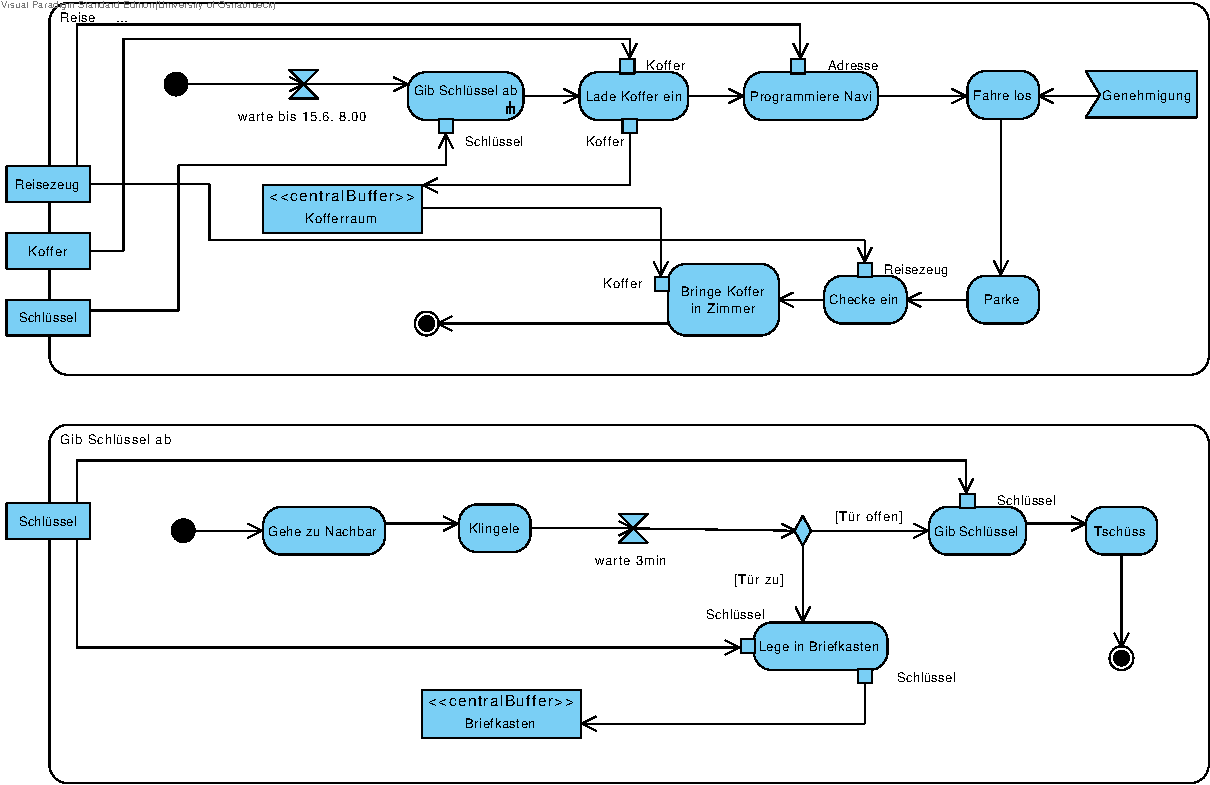
\includegraphics[width=\linewidth]{Reise.pdf}
      \caption{Aktivitätsdiagramm für Herrn Faber}
   \label{akti}}
\end{figure}

\section{Zeitdiagramm}

Für das Diagramm (\autoref{wildschwein}) nehmen wir an, dass der \texttt{Schweinebrater} immer 2
Einheiten ins Depot legt in der Zeit, die \texttt{Obelix} zum Entfernen einer
Einheit braucht (aufgrund der \texttt{sleep()}-Argumente). Nach 9 Durchläufen
ist das Depot dann voll, der \texttt{Schweinebrater} ruft \texttt{wait()} auf
und wird später geweckt. Das selbe kann natürlich auch \texttt{Obelix}
passieren, dieser Fall ist hier nicht dargestellt.

\begin{figure}
   {\centering      
   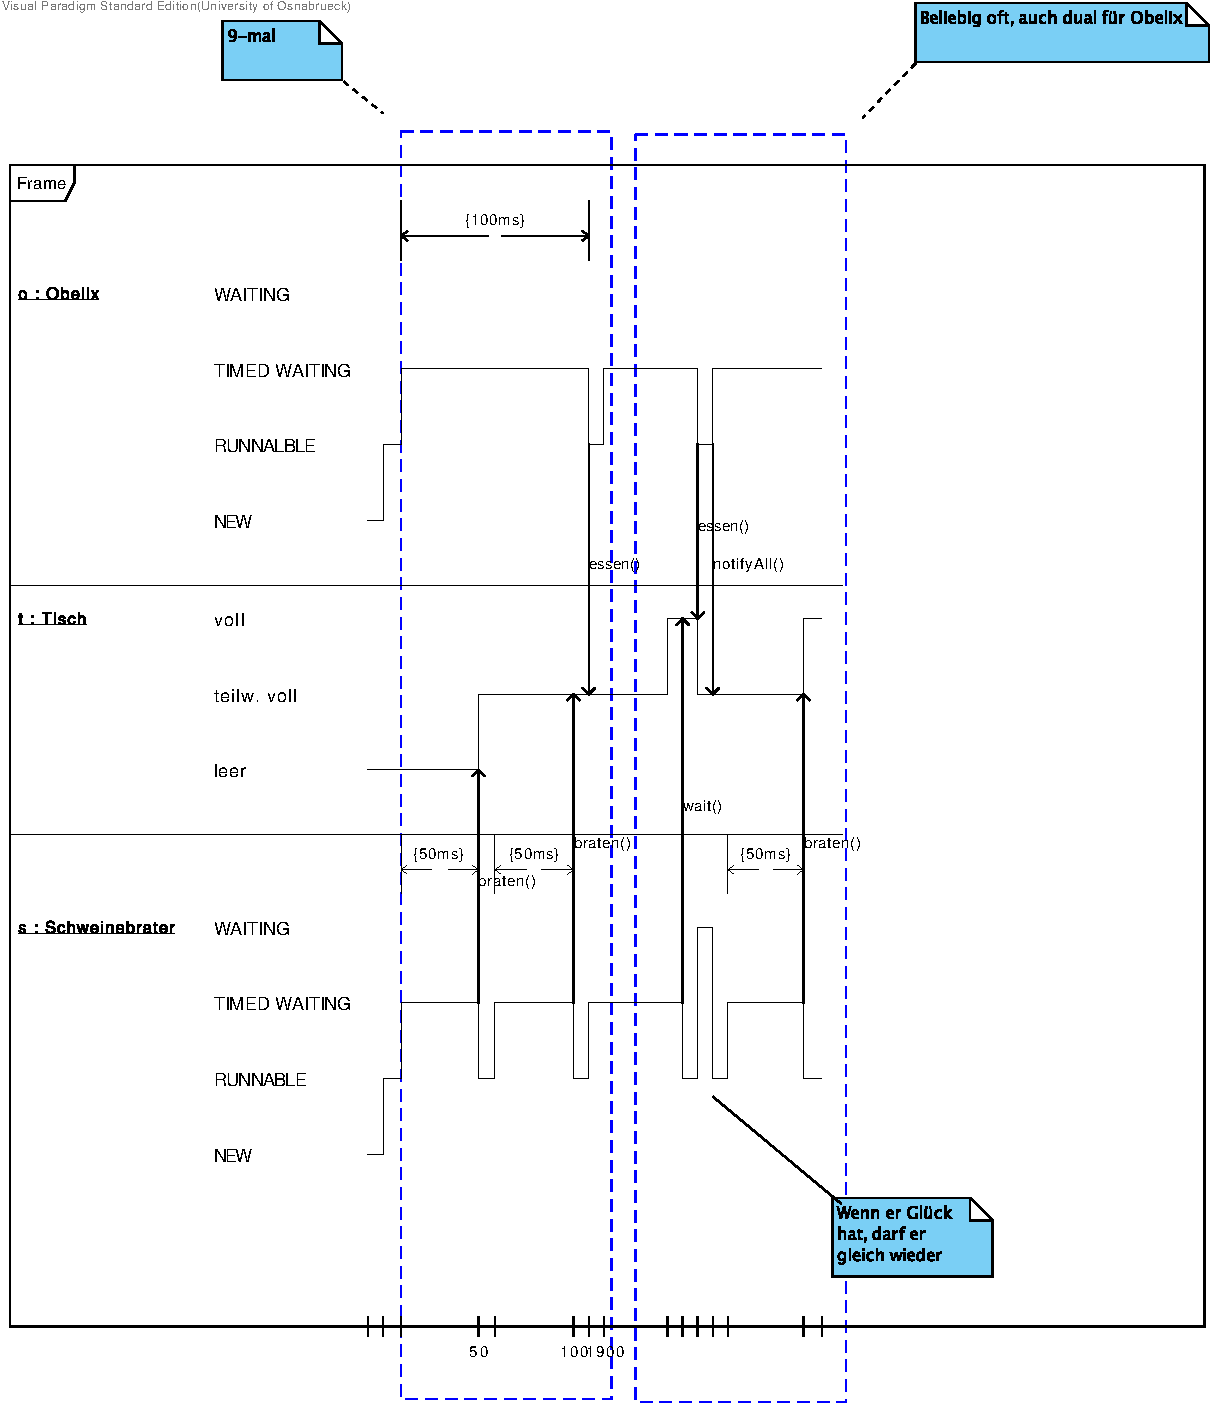
\includegraphics[width=\linewidth]{Wildschwein.pdf}
   \caption{Zeitdiagramm des Producer-Consumer-Szenarios}
   \label{wildschwein}}
\end{figure}

\section{Anwendungsfalldiagramm}

\begin{figure}
   {\centering      
   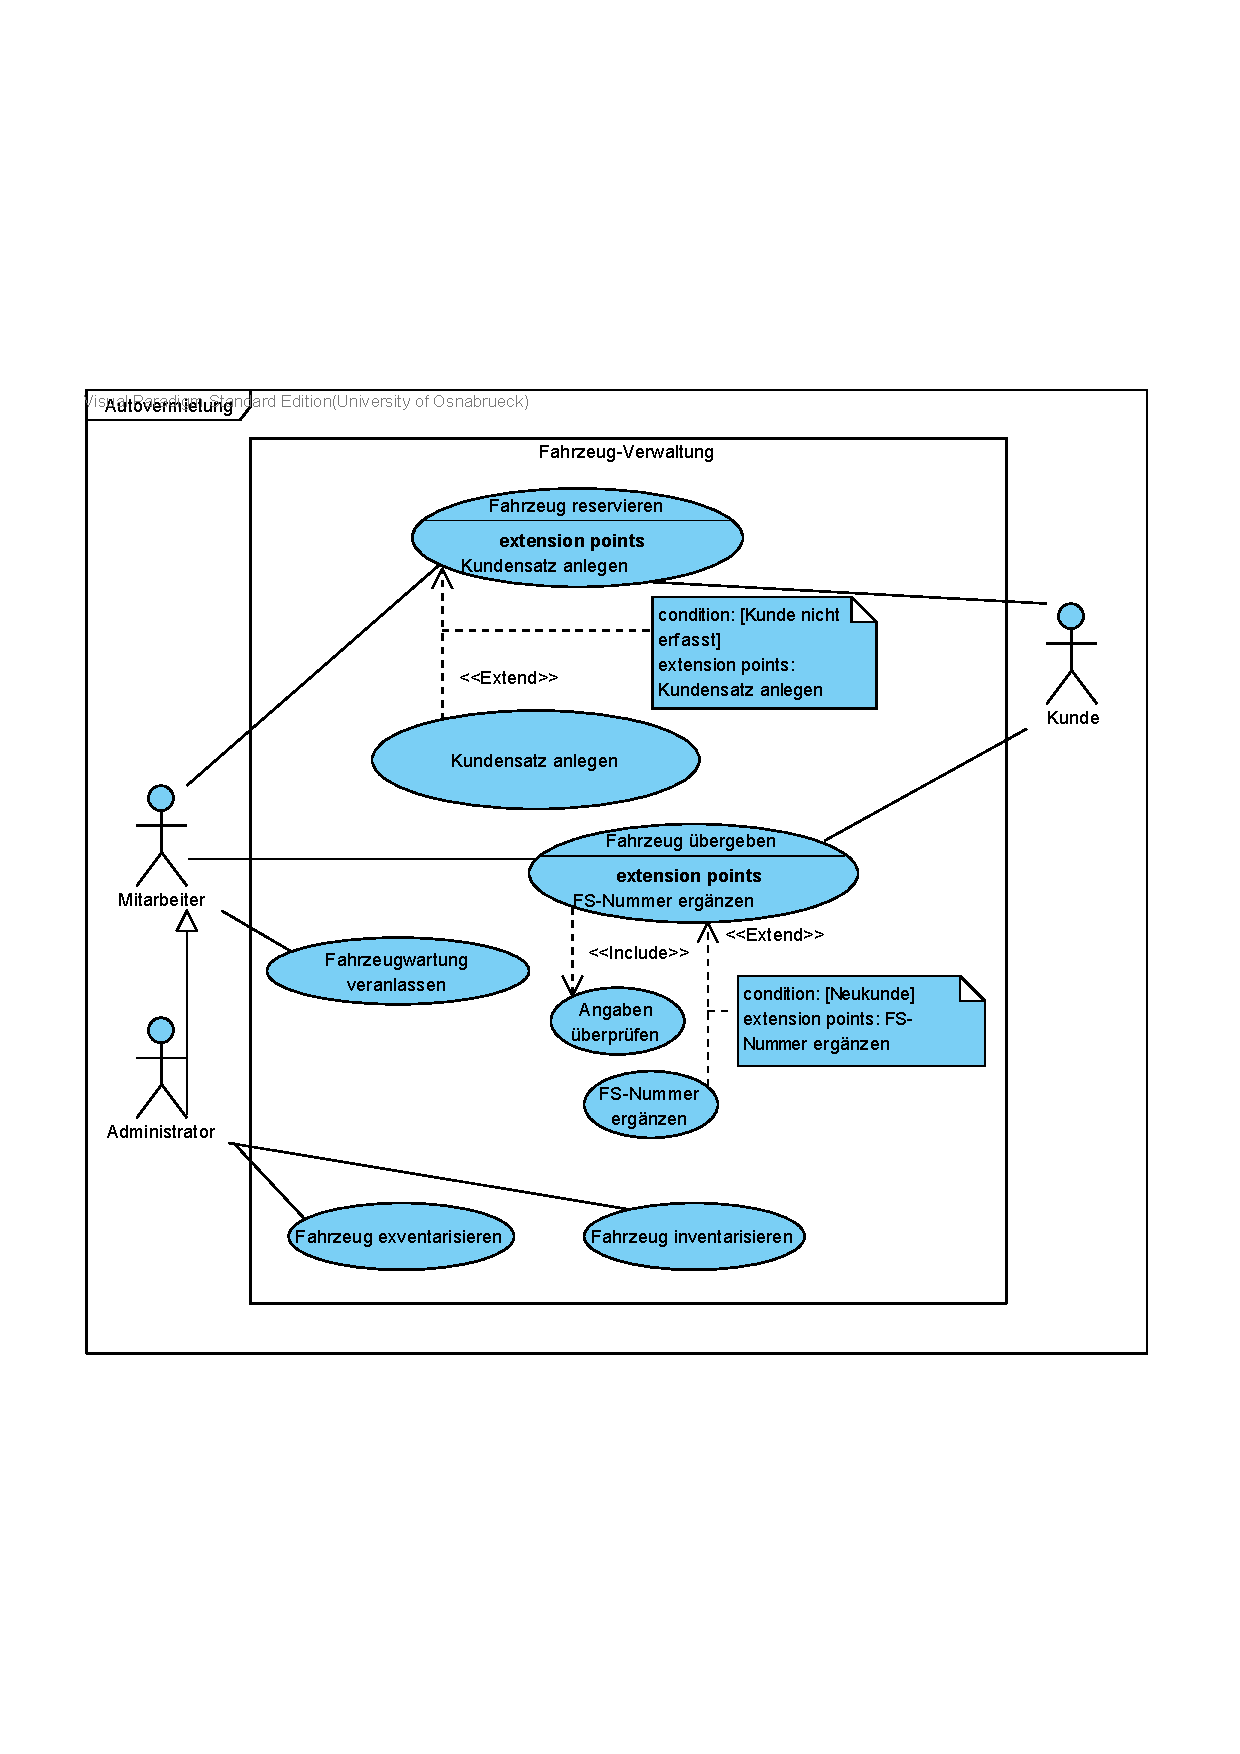
\includegraphics[width=\linewidth]{Autovermietung.pdf}
   \caption{Use-Case-Diagram der Autovermietung}
   \label{autovermietung}}
\end{figure}

\begin{table}[h]
\begin{tabular}{l | l}
\multicolumn{2}{l}{Beschreibung Anwendungsfall}                                         \\
Name                 & Fahrzeug übergeben                                               \\
Kurzbeschreibung     & (Reserviertes) Fahrzeug wird von Mitarbeiter an Kunden übergeben \\
Akteure              & Mitarbeiter, Kunde                                               \\
Auslöser             & Kunde kommt zu Abholtermin                                       \\
Ergebnis(se)         &  Fahrzeug nicht verfügbar                                                                \\
Eingehende Daten     & Führerscheinklasse, Alter, Führerscheinnummer                    \\
Vorbedingungen       & Führerscheinklasse und Alter entsprechen Anforderungen           \\
Nachbedingungen      &   -                                                               \\
Essenzielle Schritte & Angaben überprüfen, FS-Nummer ergänzen                           \\
Offene Punkte        &  -                                                                \\
Sonstige Anmerkungen & -                                                                
\end{tabular}

\caption{Beschreibung Use-Case Fahrzeug übergeben}
\end{table}


\end{document}
